\documentclass[10pt]{article}

\usepackage{parskip}
\usepackage[margin=1in]{geometry} 
\usepackage{amsmath,amsthm,amssymb, graphicx, multicol, array}
\usepackage{enumitem}
\usepackage{mathtools}
\usepackage{amssymb}
\usepackage{href-ul}
 
\newcommand{\N}{\mathbb{N}}
\newcommand{\Z}{\mathbb{Z}}
 
\newenvironment{problem}[2][Problem]{\begin{trivlist}
\item[\hskip \labelsep {\bfseries #1}\hskip \labelsep {\bfseries #2.}]}{\end{trivlist}}

\begin{document}
 
\title{Problems 2}
\author{Jakob Sverre Alexandersen\\
GRA4153 Advanced Statistics}
\maketitle

\tableofcontents
\newpage

\section{Statistics, Sufficiency, Completeness \& Ancilliarity}

1. In the context of Example 3.1, which of the following are statistics: 

\begin{enumerate}[label=(\roman*)]
    \item $\frac{1}{n} \sum_{i = 1}^{n} X_i $
    \item $\sum_{i = 1}^{n} X_i $
    \item $\frac{1}{n} \sum_{i = 1}^{n} X_i^2 $
    \item $\frac{1}{n} \sum_{i = 1}^{n} (X_i - \theta) $
    \item $\frac{1}{n} \sum_{i = 1}^{n} (X_i^2 - 1) $
\end{enumerate}

Example 3.1 states that: 

Suppose we observer $n $ samples which satisfy 

\begin{gather*}
    X_i = \theta + \epsilon_i\quad(i = 1, …, n),\quad\epsilon_1, …, \epsilon_n\text{ are i.i.d. draws from } \mathcal{N}(0, 1),\quad\theta\in\Theta\subset \mathcal{R}
\end{gather*}
Then, our statistical model is 
\begin{gather*}
    \mathcal{P} = \{\mathcal{N}(\theta, 1)^n : \theta\in\Theta\},
\end{gather*}
where $\mathcal{N}(\theta, 1)^n $ denotes the distribution of $n $ i.i.d. draws from a $\mathcal{N}(\theta, 1)$ distribution. $\triangle $

A statistic is any measurable function of the observed sample that does not depend on unknown parameters. Therefore all but (iv) are statistics, as it depends on the parameter $\theta $

\hfill

2. In the context of Example 3.1, find a minimal sufficient statistic. 

A minimal sufficient statistic is $T(X) = \sum_{i = 1}^{n} X_i $

\hfill

3. Let $X \sim \text{Poisson}(\theta) \text{ and } Y \sim \text{ Poisson}(\theta^2)$, independent, with $\theta \in (0, \infty)$. (i) Find a minimal sufficient statistic for the family of joint distributions for $Z = (X, Y)$. (ii) Is this minimal sufficient states complete?

\begin{enumerate}[label=(\roman*)]
    \item \textbf{Minimal sufficient statistic}
    
    The joint pmf is 
    \begin{gather*}
        P_\theta(X = x, Y = y) = \frac{e^{-\theta}\theta^x}{x!} \cdot \frac{e^{-\theta^2}\theta^{2y}}{y!} = \frac{1}{x!y!}e^{-(\theta + \theta^2)}\theta^{x + 2y} \\
        P_{\theta}(x, y) = h(x, y)g_\theta(T),\quad h(x,y) = \frac{1}{x!y!},\quad g_\theta(t) = e^{-(\theta + \theta^2)}\theta^t,\quad T = X + 2Y
    \end{gather*}
    By the factorization theorem, $T = X + 2Y $ is sufficient (Fisher-Neyman factorization)

    For minimal sufficiency, consider
    \begin{gather*}
        \frac{P_\theta(x, y)}{P_\theta(x', y')} = \frac{x'!y'!}{x!y!}\theta^{(x + 2y) - (x' + 2y')}
    \end{gather*}
    The ratio is free of $\theta $ iff $x + 2y = x' + 2y' $. Hence $T = X + 2Y $ is minimal sufficient (Lehmann-Scheffé minimal sufficiency criterion)
    \newpage
    \item Completeness
    
    Let $T = X + 2Y $ for $t = 0, 1, 2, … $
    \begin{gather*}
        P_\theta(T = t) = e^{-(\theta + \theta^2)}\theta^t\sum_{y = 0}^{\lfloor t / 2 \rfloor}\frac{1}{(t - 2y)!y!} = e^{-(\theta + \theta^2)}\theta^tc_t,
    \end{gather*}
    where $c_t > 0 $ (the term $y = 0 $ equals $1 / t!$)

    Assume $\mathbb{E}[g(T)] = 0 \quad\forall \theta > 0 $. Then 
    \begin{gather*}
        0 = \mathbb{E}[g(T)] = \sum_{t = 0}^{\infty}g(t)P_\theta(T = t) = e^{-(\theta + \theta^2)}\sum_{t = 0}^{\infty}g(t)c_t\theta^t,\quad\theta > 0
    \end{gather*}
    Multiplying by $e^{\theta + \theta^2}$ gives 
    \begin{gather*}
        \sum_{t = 0}^{\infty}a_t\theta^t = 0,\quad a_t = g(t)c_t,\quad\theta > 0
    \end{gather*}
    By uniqueness of power series coefficients, $a_t = 0 \quad\forall t $, hence $g(t) = 0\quad\forall t $ since $c_t > 0 $. Therefore $T $ is complete (Uniqueness of power series coefficients)
\end{enumerate}

\hfill 

4. Let $Z = (Z_1, …, Z_n)$ be i.i.d. standard normal random variables. Show that $||Z||$ and $Z / ||Z||$ are independent. [Hint: consider an appropriate model where each $Z_i $ has a normal distribution depending on some $\theta $ and use Basu's Theorem]

Model: for a scale parameter $\sigma > 0 $, consider the family $Z \sim \mathcal{N}_n(0, \sigma^2I_n)$. Define $T = ||Z||^2 $ and $U = Z / ||Z|| $ (defined on $\{Z \neq 0\}$, which has probability 1)

$T $ is complete and sufficient for $\sigma^2 $. The joint density factors as $f_\sigma(z) = (2\pi\sigma)^{-n / 2} \exp\{-||z||^2 / (2\sigma^2)\}$, so by the factorization theorem $T $ is sufficient. Moreover, $T \sim \sigma^2\chi_n^2 $, i.e., a Gamma distribution with fixed shape $n / 2 $ and scale $2 \sigma^2 $. For this one-parameter Gamma family (fixed shape), the statistic $T $ is complete.

$U $ is ancillary for $\sigma $. If $X \sim \mathcal{N}(0, I_n)$, then $Z \stackrel{d}{=} \sigma X $, and $U = Z / ||Z|| = (\sigma X) / ||\sigma X|| = X / ||X||$, so the distribution of $U $ does not depend on $\sigma $ (indeed $U $ is uniform on the unit sphere $S^{n - 1}$)

By Basu's theorem, a complete sufficient statistic is independent of any ancillary statistic. Hence $T $ and $U $ are independent for every $\sigma > 0 $. Since $||Z|| $ is a measurable function of $T $, it follows that $||Z||$ and $Z / ||Z|| $ are independent. 

Taking $\sigma = 1 $ gives the desired result for i.i.d. standard normal components.\qed 

\newpage

5. Consider the family $\{f_p : p \in [0, 1]\}$ where $f_p $ is the Bernoulli pmf of Example 2.2. Show that this is an exponential family and write it in a canonical form. 

Example 2.2 states that:

A random variable $X $ has a \textit{Bernoulli(p) distribution} if for some $p \in [0, 1]$
\[
X = 
\begin{cases}
    1\quad\text{with probability }p\\
    0\quad\text{with probability }1 - p
\end{cases},
\]
or, equivalently, its pmf is 
\[
f(x) = 
\begin{cases}
    p\quad x = 1\\
    1 - p\quad x = 0\\
    0\quad\text{otherwise}
\end{cases}.
\]

We write the Bernoulli pmf as 
\begin{gather*}
    f_p(x) = p^x(1 - p)^{1 - x}, \quad x\in \{0, 1\}, p\in (0, 1)
\end{gather*}
Then 
\begin{gather*}
    f_p(x) = \exp\{x \log p + (1 - x)\log(1 - p)\} = \exp\big\{x \log \frac{p}{1 - p} + \log(1 - p)\big\}
\end{gather*}
Let the canonical (natural) parameter be 
\begin{gather*}
    \theta = \log \frac{p}{1 - p} \iff p = \frac{e^\theta}{1 + e^\theta},
\end{gather*}
and define the log-partition function 
\begin{gather*}
    A(\theta) = \log(1 + e^\theta)
\end{gather*}
Since $A(\theta) = -\log(1 - p)$, the pmf becomes 
\begin{gather*}
    f_\theta(x) = \exp\{x\theta - A(\theta)\},\quad x \in \{0, 1\},
\end{gather*}
with base measure $h(x) \equiv 1 $ and sufficient statistic $T(x) = x $. The natural parameter space is $\Theta = \mathbb{R}$ (corresponding to $p\in (0, 1)$), with $p = 0, 1 $ as limiting cases. Therefore, the Bernoulli family is a one-parameter exponential family in canonical form. \qed

\newpage

6. Consider the family $\{p_\lambda : \lambda\in(0, \infty)\}$ where $p_\lambda $ is the Poisson pmf of Example 2.4. Show that this is an exponential family and write it in canonical form. 

Example 2.4 states that:

A random variable $X $ has a Poisson($\lambda $) distribution if it has the pmf 
\begin{gather*}
    f(x) = \frac{\exp(-\lambda)\lambda^x}{x!},\quad\text{for }x = 0, 1, …
\end{gather*}
and x otherwise. Note this places positive mass on every positive integer. The parameter $\lambda $ is called the \textit{intensity} parameter and the Poisson distribution is often used to model the number of events which occur in a fixed interval.

We write the Poisson pmf as 
\begin{gather*}
    f(x | \lambda) = \frac{\exp(-\lambda)\lambda^x}{x!} = \frac{1}{x!}\exp\{x \log \lambda - \lambda\},\quad x = 1, 2, …, \lambda > 0
\end{gather*}
This has the exponential-family form 
\begin{gather*}
    f(x | \lambda) = h(x)\exp\{\eta(\lambda)T(x) - A\big(\eta(\lambda)\big)\},
\end{gather*}
with the identifications that the sufficient statistic: $T(x) = x $, canonical parameter: $\eta(\lambda) = \log \lambda \in \mathbb{R}$, log partition: $A(\eta) = \exp(\eta)$ and base measure: $h(x) = 1 / x!$

Canonical form(using $\theta = \eta = \log \lambda $):
\begin{gather*}
    f(x | \theta) = \frac{1}{x!}\exp\{\theta x - e^\theta\},\quad\theta\in \mathbb{R}, x = 0, 1, …
\end{gather*}
Thus, the Poisson family is a (regular) one-parameter exponential family with natural parameter space $\mathbb{R}$

\newpage

\section{Statistical inference and performance criteria}

\hfill

1. Prove the Bias-Variance decomposition in Example 3.10 [Hint: The general case follows from the univariate case which can be shown by applyg Var($Z) = \mathbb{E}[Z^2] - \mathbb{E}[Z]^2 $ to $Z = T(X) - g(\theta)$]

Example 3.10 [quadratic loss] states that: 

Suppose, given some model $\mathcal{P} = \{P_\theta : \theta\in\Theta\}$, we want to estimate some $g(\theta)\in \mathcal{G}\subset \mathbb{R}^K $. One commonly used loss function is the \textit{quadratic loss}, defined for $t\in \mathbb{R}^K $ as 
\begin{gather*}
    L(\theta, t) = ||g(\theta) - t||^2.
\end{gather*}
The risk function of an estimate $T = T(X)$ under the quadratic loss is then 
\begin{gather*}
    R(\theta, T) = \mathbb{E}_{P_\theta}||g(\theta) - T(X)||^2.
\end{gather*}
This risk function is often called the \textit{mean squared error} (MSE) and satisfies a decomposition into bias and variance terms ("the bias-variance tradeoff"):
\begin{gather*}
    R(\theta, T) = \mathbb{E}_{P_\theta}||g(\theta) - T(X)||^2 = \sum_{k = 1}^{K}\text{Var}_{P_\theta}\big(T_k(X)\big) + \big(\mathbb{E}_{P_\theta}T_k(X) - g_k(\theta)\big)^2
\end{gather*}

\textbf{Proof:}

For any random variable $Z $ and constant $a $,
\begin{gather*}
    \mathbb{E}(Z - a)^2 = \text{Var}(Z) + (\mathbb{E}Z - a)^2
\end{gather*}
Then we write $T = (T_1, …, T_K)$ and $g(\theta) = \big(g_1(\theta), …, g_K(\theta)\big)$. Since the squared Euclidean norm is a sum of squares, 
\begin{gather*}
    \mathbb{E}_{P_\theta}||g(\theta) - T(X)||^2 = \sum_{k = 1}^{K}\mathbb{E}_{P_\theta}\big(T_k(X) - g_k(\theta)\big)^2
\end{gather*}
Apply the univariate identity to each component with $Z = T_k(X)$ and $a = g_k(\theta)$:
\begin{gather*}
    \mathbb{E}_{P_\theta}\big(T_k(X) - g_k(\theta)\big)^2 = \text{Var}_{P_\theta}\big(T_k(X)\big) + \big(\mathbb{E}_{P_\theta}T_k(X) - g_k(\theta)\big)^2
\end{gather*}
Summing over $k $ gives 
\begin{gather*}
    R(\theta, T) = \sum_{k = 1}^{K}\text{Var}_{P_\theta}\big(T_k(X)\big) + \big(\mathbb{E}_{P_\theta}T_k(X) - g_k(\theta)\big)^2
\end{gather*}
This is the desired bias-variance decomposition (with bias therm $\mathbb{E}_{P_\theta}T_k(X) - g_k(\theta)$ for each component).\qed
\newpage 

2. Let $X = (X_1, …, X_n)$ and consider the family $\{p_\lambda^n : \lambda\in(0,\infty)\}$ where $p_\lambda $ is the Poisson pmf of example 2.4. Consider the estimator $T(X) = X_1 $. Show that this is unbiased. Use the Rao-Blackwell Theorem to find a better estimator. [*Derive an explicit expression for the estimator.]

\textbf{Proof:}

Unbiasedness: 

Since each $X_i \sim \text{Poisson}(\lambda)$, we have $\mathbb{E}[X_1] = \lambda $. Thus $T(X) = X_1 $ is unbiased for $\lambda $.

For Rao-Blackwell we let the sufficient statistic for $\lambda $ be $S = \sum_{i = 1}^{n}X_i $ (by the factorization theorem). Then we define the Rao-Blackwellized estimator $T^*(X) = \mathbb{E}[X_1 | S]$. By exchangeability, $\mathbb{E}[X_i | S]$ is the same for all $i $, and since $\sum_{i = 1}^{n}X_i = S $, taking conditional expectations gives 
\begin{gather*}
    \sum_{i = 1}^{n}\mathbb{E}[X_i | S] = \mathbb{E}\left[\sum_{i = 1}^{n}X_i | S\right] = S,
\end{gather*}
hence $\mathbb{E}[X_1 | S] = S/n $. (equivalently, using the standard result that given $S = s, (X_1, …, X_n) | S = s \sim\text{Multinomial}(s;1 / n, …, 1 / n)$, so $X_1 | S = s \sim \text{Binomial}(s, 1 / n)$ and $\mathbb{E}[X_1 | S = s] = s / n $)

Therefore, the Rao-Blackwell estimator is 
\begin{gather*}
    \hat{\lambda}_{\text{RB}}(X) = \mathbb{E}[X_1 | S] = \frac{S}{n} = \bar{X}
\end{gather*}
with the following properties: \qed
\begin{itemize}
    \item Unbiased: $\mathbb{E}[\hat{X}] = \lambda $
    \item Lower variance: $\text{Var}(X_1) = \lambda $ while $\text{Var}(\hat{X}) = \lambda / n $, so for $n > 1 $ the Rao-Blackwell estimator is strictly better 
    \item In fact, since $S \sim \text{Poisson}(n\lambda)$ is complete and sufficient, $\bar{X}$ is the UMVU (uniformly minimum-variance unbiased) estimator of $\lambda $
\end{itemize}

\newpage 

3. In the setting of Example 2.12, show that $a = (n + 2) / (n + 1)$ minimises $R(\theta, \delta_a)$. Calculate the bias of the corresponding estimator $\delta_a $

Example 2.12 [Multivariate Normal] says that: 

A random vector $X = (X_1, …, X_K)$ has the multivariate normal distribution with mean vector $\mathbb{E}X = \mu $ and a positive definite variance matrix $\mathbb{E}(X - \mu)(X - \mu)' = \Sigma $ if its joint pdf is 
\begin{gather*}
    f(x) = \det(2\pi\Sigma)^{-1 / 2}\exp\left(-\frac{1}{2}(x - \mu)'\Sigma^{-1}(x - \mu)\right)
\end{gather*}
If $X = (X_1, …, X_k)$ is multivariate normally distributed, then each $X_k $ is marginally normally distributed. The converse is not necessarily true. It does hold in the special case that $X_1, …, X_K $ are independent.

\textbf{Q}: What is the estimator here? Which risk function are we using?

\hfill 

4. In the setting of Example 2.13 show that conditional on $T = t, X_1 = t $ with probability $1 / n $ and $X_1 $ is uniformly distributed on $(0, t)$ with probability $(n - 1) / n $

Example 2.13 says that: 

Let $X_n $ be a random variable with $P(X_n = n) = 1 / n $ and $P(X_n = 0) = 1 - 1 / n $. Then $X_n \xrightarrow{P} 0 $ (hence also weakly) [Exercise] but $\mathbb{E}X_n = n \times 1 / n = 1 $ for each $n $.

Let $X_1, …, X_n $ be i.i.d. Uniform(0, 1) and let $T = \max\{X_1, …, X_n\}$. Dix $0 < t < 1 $. We compute the regular conditional law of $X_1 $ given $T = t $ by a small-interval argument.

Denominator: For small $h > 0: $
\begin{gather*}
    P(t < T \le t + h) = P(\text{at least one }X_i \in (t, t + h], \text{ others }\le t) = nt^{n - 1}h + o(h),
\end{gather*}
since the density of $T $ at $t $ is $nt^{n - 1}$.

Continuous part on $(0, t)$: For $0 \ge x < t $,
\begin{gather*}
    P(X_1 \le x, t < T \le t + h) = P(X_1 \le x, \max(X_2, …, X_n)\in(t, t + h]) = (n - 1)xt^{n - 2}h + o(h),
\end{gather*}
because $X_1 \le x $ contributes factor $x $, one of $X_2, …, X_n $ lands in $(t, t + h]$ (probability $\approx (n - 1)t^{n - 2}h$), and the change of two or more in $(t, t + h]$ is $o(h) $

Hence, for $0 \le x < t $,
\begin{gather*}
    P(X_1 \le x | T \in (t, t + h]) \to \frac{(n - 1)xt^{n - 2}}{nt^{n - 1}} = \frac{n - 1}{n} \frac{x}{t} \text{ as }h \to 0
\end{gather*}
Thus the conditional law of $X_1 $ on $(0, t)$ has density $\frac{n - 1}{n} \cdot \frac{1}{t}$, i.e., Uniform(0, t) with weight $(n - 1) / n $

Atom at $t $: Also,
\begin{gather*}
    P(X_1\in (t, t + h], t < T \le t + h) = P(X_1\in (t, t + h], X_2, …, X_n \le t) = t^{n - 1}h + o(h),
\end{gather*}
so
\begin{gather*}
    P(X_1\in (t, t + h] | T \in (t, t + h]) \to \frac{t^{n - 1}}{nt^{n - 1}} = \frac{1}{n}.
\end{gather*}
This yields $P(X_1 = t | T = t) = 1 / n $

Therefore, conditional on $T = t, X_1 $ equals $t $ with probability $1 / n $, and with the remaining probability $(n - 1) / n $ it is Uniform(0, $t$).\qed

\newpage  

5. Consider a random sample $X = (X_1, …, X_n)$ where each $X_i \sim \mathcal{N}(\mu, \sigma^2)$. Calculate the information matrix $I(\theta)$ where $\theta = (\mu, \sigma^2)$ and obtain UMVU estimators for $\mu $ and $\sigma^2 $ respectively. 

We need to find the log-likelihood for one observation: 
\begin{gather*}
    \ell(\mu, \sigma^2; x) = -\frac{1}{2}\log(2\pi\sigma^2) - \frac{(x - \mu)^2}{2\sigma^2}
\end{gather*}
For the sample of size $n $:
\begin{gather*}
    \ell(\mu, \sigma^2; X) = -\frac{n}{2}\log(2\pi\sigma^2) -\frac{1}{2\sigma^2}\sum_{i = 1}^{n}(X_i - \mu)^2
\end{gather*}
Scores:
\begin{gather*}
    \frac{\partial\ell}{\partial\mu} = \frac{1}{\sigma^2}\sum_{i = 1}^{n}(X_i - \mu), \quad \frac{\partial\ell}{\partial(\sigma^2)} = -\frac{n}{2\sigma^2} + \frac{1}{2\sigma^4}\sum_{i = 1}^{n}(X_i - \mu)^2
\end{gather*}
Expected Fisher information matrix $I(\theta) = \mathbb{E}[\text{Hessian}(\ell)]$:
\begin{gather*}
    I_{\mu\mu} = -\mathbb{E}\left[\frac{\partial^2\ell}{\partial\mu^2}\right] = \frac{n}{\sigma^2}\\
    I_{\mu,\sigma^2} = -\mathbb{E}\left[\frac{\partial^2\ell}{\partial\mu\partial(\sigma^2)}\right] = 0\\
    I_{\sigma^2,\sigma^2} = -\mathbb{E}\left[\frac{\partial^2\ell}{\partial(\sigma^2)^2}\right] = \frac{n}{2\sigma^4}\\
\end{gather*}
Thus,
\begin{gather*}
    I(\theta) = \begin{pmatrix}
        \frac{n}{\sigma^2} & 0 \\
        0 & \frac{n}{2\sigma^4}
    \end{pmatrix}
\end{gather*}
UMVU estimators:
\begin{itemize}
    \item The statistic $(\overline{X}, S^2)$ with $\overline{X} = \frac{1}{n}\sum X_i $ and $S^2 = \frac{1}{n - 1}\sum (X_i - \overline{X})^2 $ is sufficient and complete for $(\mu, \sigma^2)$ (for $n \ge 2 $) in the normal family.
    \item Since $\mathbb{E}[\overline{X}] = \mu $ and $\mathbb{E}[S^2] = \sigma^2 $, by Lehmann-Scheffé, the UMVU estimators are 
    \begin{itemize}
        \item for $\mu: \hat{\mu}_{\text{UMVU}} = \overline{X}$
        \item for $\sigma^2: \widehat{\sigma^2}_{\text{UMVU}} = S^2$
    \end{itemize}
\end{itemize}
\qed

\newpage 

6. Suppose $p_\theta $ is a pdf for each $\theta $, that (i) of Theorem 3.7 holds and that $p_\theta $ can be twice differentiated under the integral sign in that 
\begin{gather*}
    \nabla_\theta\nabla_{\theta'}\int p_\theta(x) dx = \int\nabla_\theta\nabla_{\theta'}p_\theta(x) dx
\end{gather*}
Show that $-I(\theta) = \mathbb{E}_{P_\theta}[\nabla_{\theta'}\ell_\theta]$. This is called the \textit{information equality}.

Theorem 3.7 [The information inequality] states:

\textit{Suppose that X has a distribution in the dominated model }$\mathcal{P} = \{P_\theta : \theta\in\Theta\}$\textit{ with }$\Theta\in \mathbb{R}^K $\textit{ let }$\ell_\theta := \nabla_\theta\log p_\theta $. \textit{ If  }$\delta $ \textit{ is any (real-valued) statistic with }$\mathbb{E}_{P_\theta}\delta(X)^2 < \infty $ \textit{ and:}
\begin{enumerate}[label=(\roman*)]
    \item $\ell_\theta $ \textit{ exists, }$\mathbb{E}_{P_\theta}\ell_\theta(X) = 0 $ \textit{ and }$I(\theta) := \mathbb{E}_{P_\theta}[\ell_\theta(X)\ell_\theta(X)']$ \textit{ exists and is positive definite,}
    \item $\nabla_\theta \mathbb{E}_{P_\theta}[\delta(X)]$\textit{ exists and satisfies }$\nabla_\theta \mathbb{E}_{P_\theta}[\delta(X)] = \int\nabla_\theta\delta(x)p_\theta(x) dx $,
\end{enumerate}
\textit{then}
\begin{gather*}
    \text{Var}_{P_\theta}\big(\delta(X)\big) \ge \big(\nabla_\theta \mathbb{E}_{P_\theta}[\delta(X)]\big)'I(\theta)^{-1}\big(\nabla_\theta \mathbb{E}_{P_\theta}[\delta(X)]\big)
\end{gather*}

\textbf{Proof:}

Let $\ell_\theta(x) := \nabla_\theta\log p_\theta(x)$. For each $x $ with $p_\theta(x) > 0 $, the Hessian of the log-density satisfies the standard identity (by the quotient rule for vector derivatives):
\begin{gather*}
    \nabla_\theta\ell_\theta(x) = \nabla_{\theta'}\nabla_\theta\log p_\theta(x) = \frac{\nabla_{\theta'}\nabla_\theta p_\theta(x)}{p_\theta(x)} = \frac{\nabla_\theta p_\theta(x)\nabla_{\theta'}p_\theta(x)}{p_\theta(x)^2} = \frac{\nabla_{\theta'}\nabla_\theta p_\theta(x)}{p_\theta(x)} = -\ell_\theta(x)\ell_\theta(x)'
\end{gather*}
Taking expectation under $P_\theta $ and using the given interchange of differentiation and integration,
\begin{gather*}
    \mathbb{E}_{P_\theta}[\nabla_{\theta'}\ell_\theta(X)] = \int \left(\frac{\nabla_{\theta'}\nabla_\theta p_\theta(x)}{p_\theta(x)} -\ell_\theta(x)\ell_\theta(x)'\right)p_\theta(x) dx = \int \nabla_{\theta'}\nabla_\theta p_\theta(x) dx - \mathbb{E}[\ell_\theta(X)\ell_\theta(X)']
\end{gather*}
By normalization and the assumed twice-differation under the integral sign,
\begin{gather*}
    \int \nabla_{\theta'}\nabla_\theta p_\theta(x) dx = \nabla_{\theta'}\nabla_\theta \int p_\theta(x) dx = \nabla_{\theta'}\nabla_\theta1 = 0
\end{gather*}
Hence 
\begin{gather*}
    \mathbb{E}_{P_\theta}[\nabla_{\theta'}\ell_\theta(X)] = - \mathbb{E}[\ell_\theta(X)\ell_\theta(X)'] = - I(\theta),
\end{gather*}
which is the information equality \qed

\newpage 

7. Suppose that $S(X)$ is a confidence set for $g(\theta)$ s.t. $P_\theta\big(g(\theta)\in S(X)\big) = 1 - \alpha \quad\forall\theta\in\Theta$ Form a test, $\varphi $, as in (21). What is the size of $\varphi $?

The test in (21) is described as:
\[
\varphi(x) :=
\begin{cases}
    1\quad\text{when }g_0\notin S(X)\\
    0\quad\text{otherwise}
\end{cases}
\]
Size of $\varphi: \alpha $

\textbf{Proof: }

For any $\theta $ with $g(\theta) = g_0 $,
\begin{gather*}
    P_\theta\big(\varphi(X) = 1\big) = P_\theta\big(g_0\notin S(X)\big) = 1 - P_\theta\big(g_0\in S(X)\big) = 1 - P_\theta\big(g(\theta) \in S(X)\big) =\alpha,
\end{gather*}
since $S(X)$ has exact coverage $1 - \alpha \quad\forall\theta $. Thus 
\begin{gather*}
    \sup_{\theta : g(\theta) = g_0}P_{\theta}\big(\varphi(X) = 1\big) = \alpha
\end{gather*}
\qed

8. Show: $k_\alpha $ is the $1 - \alpha $ quantile of the $\chi^2(1)$ distribution iff $k_\alpha^{1/2}$ is the $1 - \alpha / 2 $ quantile of the $\mathcal{N}(0, 1)$ distribution.

\textbf{Proof:}

Let $Z \sim \mathcal{N}(0, 1) $ and note that $Z^2 \sim\chi^2(1)$

For $k \ge 0 $,
\begin{gather*}
    P\big(\chi^2(1) \le k\big) = P(Z^2\le k) = P(-\sqrt{k}\le Z \le \sqrt{k}) = \Phi(\sqrt{k}) - \Phi(-\sqrt{k})= 2\Phi(\sqrt{k}) - 1,
\end{gather*}
where $\Phi $ is the standard normal cdf. 

Thus, $k_\alpha $ is the $1 - \alpha $ quantile of $\chi^2(1) $ iff 
\begin{gather*}
    2\Phi(\sqrt{k_\alpha}) - 1 = 1 - \alpha \iff \Phi(\sqrt{k_\alpha}) = 1 - \alpha / 2
\end{gather*}
Since $\Phi $ is strictly increasing, this is equivalent to 
\begin{gather*}
    \sqrt{k_\alpha} = \Phi^{-1}(1 - \alpha / 2),
\end{gather*}
i.e., $\sqrt{k_\alpha}$ is the $1 - \alpha / 2 $ quantile of $\mathcal{N}(0, 1)$\qed

\newpage 

9. Verify the form of $S(X) $ in Example 3.15

Example 3.15 states: 

Suppose we are interested in the mean of $X \sim \mathcal{N}(\mu, \sigma^2)$ with known $\sigma^2 $. In particular, let's suppose we want to construct a $1 - \alpha $ confidence set for $\mu $. The set $S(X) = \{a : \phi_a (X) = 0\}$ is a $1 - \alpha $ confidence set for $\mu $. Let's describe this set in a more straightforward way. Note that 
\begin{gather*}
    \phi_a(X) = 0 \iff T \le k_\alpha \iff T^{1 / 2} \le k_\alpha^{1 / 2} \text{ or } -T^{1 / 2} \le k_\alpha^{1 / 2}
\end{gather*}
Here we note that $c_\alpha := k_\alpha^{1 / 2}$ is the $1 - \alpha / 2 $ quantile of a standard normal r.v. Since $T^{1 / 2} = \frac{(X - a)}{\sigma}$ this gives our set as 
\begin{gather*}
    S(X) = [X - \sigma c_\alpha, X + \sigma c_\alpha]
\end{gather*}
Claim: for $X \sim \mathcal{N}(\mu, \sigma^2)$ with known $\sigma^2 $, the inverted acceptance region yields 
\begin{gather*}
    S(X) = \{a : \phi_a(X) = 0\} = [X - \sigma c_\alpha, X + \sigma c_\alpha]
\end{gather*}
where $c_\alpha := k_\alpha^{1 / 2}$ is the $1 - \alpha / 2 $ standard normal quantile

\textbf{Proof:}

Under $H_0: \mu = a $, the standardized statistic 
\begin{gather*}
    Z = \frac{X - a}{\sigma} \sim \mathcal{N}(0, 1)
\end{gather*}
so $T = Z^2 = \frac{(X - a)^2}{\sigma^2} \sim\chi_1^2 $ [standard result: if $Z \sim \mathcal{N}(0, 1)$ then $Z^2 \sim\chi_1^2 $]

A level-$\alpha $ two-sided test based on $T $ rejects $T $ for $T > k_\alpha $, where $k_\alpha $ is the $(1 - \alpha)$ quantile of $\chi_1^2 $. Hence 
\begin{gather*}
    \phi_a(X) = 0 \iff T \le k_\alpha \iff \frac{(X - a)^2}{\sigma^2} \le k_\alpha \iff |X - a| \le \sigma\sqrt{k_\alpha}
\end{gather*}
Let $c_\alpha = \sqrt{k_\alpha}$. Since $Z \sim \mathcal{N}(0, 1)$,
\begin{gather*}
    \mathbb{P}(|Z| \le c_\alpha) = \mathbb{P}(Z^2 \le k_\alpha) = 1 - \alpha \iff 2\Phi(c_\alpha) - 1 = 1 - \alpha \iff \Phi(c_\alpha) = 1 - \frac{\alpha}{2}
\end{gather*}
so $c_\alpha = z_{1 - \alpha / 2}$. Therefore
\begin{gather*}
    \phi_\alpha(X) = 0 \iff -\sigma c_\alpha \le X - a \le \sigma c_\alpha \iff a \in [X - \sigma c_\alpha, X + \sigma c_\alpha]
\end{gather*}
which verifies the standard form. \qed

\newpage

\section{Asymptotic statistics}

\hfill 

1. Prove Proposition 3.4 [Hint: Example 3.10 may be useful]

Proposition 3.4 states:

\textit{If $(\hat{\delta}_n)_{n\in \mathbb{N}}$ is a sequence of estimators s.t. $b(\theta) := \mathbb{E}_{P_\theta}\hat{\delta}_n - g(\theta)\to 0 $ and } $\text{Var}_{P_\theta}(\hat{\delta}_n)\to 0 $ \textit{ as $n \to \infty $ for each $\theta\in\Theta $, then $\hat{\delta}_n \xrightarrow{P_\theta}g(\theta)$}

Example 3.10 [quadratic loss] states that: 

Suppose, given some model $\mathcal{P} = \{P_\theta : \theta\in\Theta\}$, we want to estimate some $g(\theta)\in \mathcal{G}\subset \mathbb{R}^K $. One commonly used loss function is the \textit{quadratic loss}, defined for $t\in \mathbb{R}^K $ as 
\begin{gather*}
    L(\theta, t) = ||g(\theta) - t||^2.
\end{gather*}
The risk function of an estimate $T = T(X)$ under the quadratic loss is then 
\begin{gather*}
    R(\theta, T) = \mathbb{E}_{P_\theta}||g(\theta) - T(X)||^2.
\end{gather*}
This risk function is often called the \textit{mean squared error} (MSE) and satisfies a decomposition into bias and variance terms ("the bias-variance tradeoff"):
\begin{gather*}
    R(\theta, T) = \mathbb{E}_{P_\theta}||g(\theta) - T(X)||^2 = \sum_{k = 1}^{K}\text{Var}_{P_\theta}\big(T_k(X)\big) + \big(\mathbb{E}_{P_\theta}T_k(X) - g_k(\theta)\big)^2
\end{gather*}

\textbf{Proof:} (using the bias-variance decomposition and Markov/Chebyshev)

Fix any $\theta\in\Theta $ and write $b_n(\theta) := \mathbb{E}_{P_\theta}\hat{\delta}_n - g(\theta)$. By the quadratic-loss risk decomposition, for $K = 1 $,
\begin{gather*}
    \mathbb{E}_{P_\theta}\big(\hat{\delta}_n - g(\theta)\big)^2 = \text{Var}_{P_\theta}(\hat{\delta}_n) + \big(b_n(\theta)\big)^2
\end{gather*}
By assumption, $\text{Var}_{P_\theta}(\hat{\delta}_n) \to 0 $ and $b_n(\theta) \to 0 $, hence 
\begin{gather*}
    \mathbb{E}_{P_\theta}\big(\hat{\delta}_n - g(\theta)\big)^2 \longrightarrow 0
\end{gather*}
For any $\epsilon > 0 $, apply Markov's inequality to the nonnegative r.v. $\big(\hat{\delta}_n - g(\theta)\big)^2 $:
\begin{gather*}
    P_\theta(|\hat{\delta}_n - g(\theta)| > \epsilon) \le \frac{\mathbb{E}\big(\hat{\delta}_n - g(\theta)\big)^2}{\epsilon^2} \longrightarrow 0
\end{gather*}
which is exactly $\hat{\delta}_n \xrightarrow{P_\theta} g(\theta)$ (Markov's inequality) \qed

\newpage 

2. Suppose that $X_1, …, X_n $ are i.i.d. Poisson($\lambda $) random variables. Show that $\hat{\lambda}_n = \frac{1}{n}\sum_{i = 1}^{n}X_i $ is consistent for $\lambda $.

\textbf{Proof:}

Let $\hat{\lambda}_n = \frac{1}{n}\sum_{i = 1}^{n}X_i $ with $X_i \overset{\text{i.i.d.}}{\sim}\text{Poisson}(\lambda)$. Then 
\begin{gather*}
    \mathbb{E}[\hat{\lambda}_n] = \frac{1}{n}\sum_{i = 1}^{n}\mathbb{E}[X_i] = \lambda\\
    \text{Var}(\hat{\lambda}_n) = \frac{1}{n^2}\sum_{i = 1}^{n}\text{Var}(X_i) = \frac{1}{n^2}\cdot n\lambda = \frac{\lambda}{n}
\end{gather*}
For any $\epsilon > 0 $, by Chebyshev's inequality,
\begin{gather*}
    P(|\hat{\lambda}_n - \lambda| \ge \epsilon) \le \frac{\text{Var}(\hat{\lambda}_n)}{\epsilon^2} = \frac{\lambda}{n\epsilon^2} \to 0
\end{gather*}
Hence, $\hat{\lambda}_n \xrightarrow{P}\lambda $, so $\hat{\lambda}_n $ is consistent for $\lambda $ (Chebyshev inequality). \qed

\hfill 

3. Draw some large integer $n $ samples from (i) a standard normal distribution and (ii) from a Cauchy distribution. Plot the cumulative sample average over $1, …, n $ (i.e. plot $X_1, (X_1 + X_2) / 2, (X_1 + X_2 + X_3) / 3, …, n^{-1}\sum_{i = 1}^{n}X_i $). Describe the observed behaviour and whether the sequence appears to follow the WLLN. If not, why not?

Normal case: The running mean $\bar{X}_n = n^{-1}\sum_{i = 1}^{n}X_i $ stabilizes near 0 and the fluctuation shrinks and grows. This is consistent with the Weak Law of Large Numbers: For i.i.d. variables with finite means, $\bar{X}\xrightarrow{P} \mathbb{E}[X]$. For $X \sim \mathcal{N}(0, 1), \mathbb{E}[X] = 0 $, so the WLLN holds. In fact, by the Strong Law, the convergence is a.s., and typical deviations are on the order of $1 / \sqrt{n}$ by the CLT.

Cauchy case: The running mean does not settle down; instead it exhibits occasional large jumps that can dramatically change the average even at large $n $. The WLLN requires a finite expectation, but the Cauchy distribution has no mean (the expectation is undefined), so the WLLN does not apply. In fact, the Cauchy is 1-stable, so for i.i.d. standard Cauchy variables, the average $\bar{X}_n $ has the same Cauchy distribution for every $n $, and therefore does not concentrate around any constant and does not converge in probability.

\begin{center}
    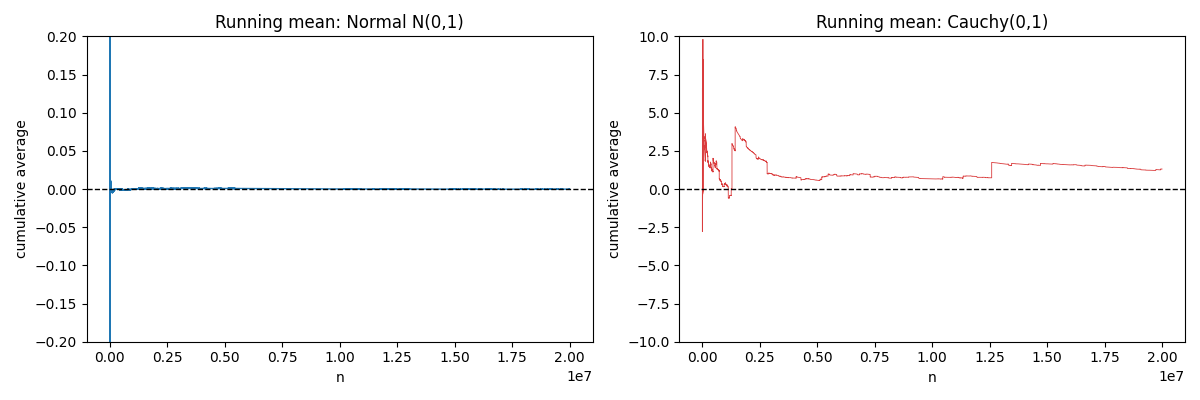
\includegraphics[width=1\textwidth]{image.png}
\end{center}

\newpage 

4. In Example 3.18 show that $s_n^2\xrightarrow{P}\sigma^2 $

Example 3.18 [Standard error of the mean] states: 

Let $V = \sigma^2 $. Whilst this is unknown, we can estimate it. If $\hat{\mu}_n := \frac{1}{n}\sum_{i = i}^{n}X_i $, then $s^2_n = \frac{1}{n}\sum_{i = i}^{n}(X_i - \hat{\mu}_n)^2 \xrightarrow{P}\sigma^2 $

Assume $X_1, …, X_n $ are i.i.d. with $\mathbb{E}X_1 = \mu $ and Var$(X_1) = \sigma^2 < \infty $, and let $\bar{X}_n = \frac{1}{n}\sum_{i = i}^{n}X_i $ and $ s_n^2 = \frac{1}{n}\sum_{i = i}^{n}(X_i - \bar{X}_n)^2 $

Key identity: 
\begin{gather*}
    s_n^2 = \frac{1}{n}\sum_{i = i}^{n}(X_i - \mu)^2 - (\bar{X}_n - \mu)^2
\end{gather*}
This follow by expanding $(X_i - \bar{X}_n)^2 = \big(X_i - \mu - (\bar{X}_n - \mu)\big)^2 $ and simplifying the cross term using $\frac{1}{n}\sum_{i = i}^{n}(X_i - \mu) = \bar{X}_n - \mu $

By the WLLN, $\frac{1}{n}\sum_{i = i}^{n}(X_i - \mu)^2 \xrightarrow{P} \mathbb{E}(X_1 - \mu)^2 = \sigma^2 $, also by the WLLN, $\bar{X}_n \xrightarrow{P}\mu $, hence by the Continuous Mapping Theorem, $(\bar{X}_n - \mu)^2 \xrightarrow{P}0 $

Therefore, by Slutsky's Theorem 

\begin{gather*}
    s_n^2 = \left(\frac{1}{n}\sum_{i = i}^{n}(X_i - \mu)^2\right) - (\bar{X}_n - \mu)^2 \xrightarrow{P}\sigma^2 - 0 = \sigma^2
\end{gather*}
\qed 

\hfill 

5. Compare the (asymptotic) $t $-test defined in (27) to the test developed in Example 3.14:

The test in (27) is described as: 

We compare $|t_n|$ to the $1 - \alpha / 2 $ quantile, $c = \Phi^{-1}(1 - \alpha / 2)$, of the standard normal distribution: we reject if 
\begin{gather*}
    |t_n| > c
\end{gather*}

The test developed in Example 3.14 is described as: 

Suppose we observe $X \sim \mathcal{N}(\mu, \sigma^2)$ where $\sigma $ is known and we want to test $H_0: \mu = a $. Let's design a test of level $\alpha $ and compute its power. 

Let $T = (X - a)^2 / \sigma^2 $. We will set our test equal to $\phi(X) = \mathbf{1}\{T > k_\alpha\}$ for a \textit{critical value }$k_\alpha $ chosen such that the test is of level $\alpha $

Using properties of the normal distribution, we have that, under $H_0 $ (i.e. if $\mu = a $) then 
\begin{gather*}
    T^{1 / 2} = (X - a) / \sigma \sim \mathcal{N}(0, 1)
\end{gather*}
Hence $T \sim\chi_1^2 $. We will take $k_\alpha $ equal to the $1 - \alpha $ quantile of the $\chi_1^2 $ distribution. This is exactly the number such that $P(T > k_\alpha) = \alpha $ if $T \sim\chi_1^2 $

In the normal, known-$\sigma $ case, the two tests are the same test in different disguises. Writing $t = (X - a) / \sigma $, Example 3.14 uses $T = t^2 $ and rejects when $T > k_\alpha $ with $k_\alpha = \chi_{1, 1-\alpha}^2 = \big(\Phi^{-1}(1 - \alpha / 2)\big)^2 = c^2 $, which is equivalent to rejecting when $|t| > c $, exactly the rejection rule in (27). The difference is that the example is an exact finite-sample test (indeed the LRT), whereas (27) is an asymptotic test meant for general estimators and estimated standard errors. 

\newpage 

6. Fill in the missing details in the proof of Proposition 3.5

\textsc{Proposition 3.5}: \textit{Suppose that (23) holds and g is continuously differentiable with full row rank Jacobian G. Then, under the null $H_0 : g(\theta) = 0 $,}


\begin{gather*}
    (23): \Bigg[ \sqrt{n}(\hat{\theta}_n - \theta) \xrightarrow{D}\mathcal{N}(0, V), \quad \hat{V}_n\xrightarrow{P}V\Bigg]
\end{gather*}

\begin{gather*}
    W_n\xrightarrow{D}\chi_p^2,
\end{gather*}
\textit{and the sequence of tests which reject when $W_n > k_\alpha $ for $k_\alpha $ the $1 - \alpha $ quantile of the $\chi_p^2 $ distribution has asymptotic size $\alpha $:}

\begin{gather*}
    \lim_{n\to\infty}P(W_n > k_\alpha) = \alpha
\end{gather*}
\textit{Under any fixed alternative, $H_1 : g(\theta) = \mathfrak{g}\neq 0 $, the test is consistent:}
\begin{gather*}
    \lim_{n\to\infty}P(W_n > k_\alpha) = 1
\end{gather*}

\textbf{Proof:} By (23), the Delta method, continuity of $G(\theta)$, the continuous mapping theorem, and Slutsky's theorem, (29) holds.

\begin{gather*}
    (29):\Bigg[W_n \xrightarrow{D}\chi_p^2\Bigg]
\end{gather*}
Since $G(\theta)$ has full row rank and $V $ is full rank, it follows that $G(\theta)VG(\theta)' $ is full rank [Exercise] and hence invertible. Therefore, by the continuous mapping theorem and Slutsky's theorem we have 
\begin{gather*}
    \left[G(\hat{\theta}_n)\hat{V}_nG(\hat{\theta}_n)'\right]^{-1/ 2}\sqrt{n}\big(g(\hat{\theta}_n) - g(\theta)\big) \xrightarrow{D}Z\sim \mathcal{N}(0, I_p).
\end{gather*}
First we handle the case under the null $g(\theta) = 0 $. This condition implies that \\$Z_n := \sqrt{n}\big[G(\hat{\theta}_n)\hat{V}_nG(\hat{\theta}_n)'\big]^{-1 / 2}g(\hat{\theta}) \xrightarrow{D}Z $. As $x \mapsto x'x $ is continuous, applying the continuous mapping theorem we obtain [Exercise]
\begin{gather*}
    W_n = Z_n'Z_n\xrightarrow{D}Z'Z\sim\chi_p^2
\end{gather*}
Moreover, since $W_n $ is an r.v., weak convergence is equivalent to convergence of its CDF at all continuity points of the limiting CDF. Here the limit is $\chi_p^2 $ which has a continuous CDF on $\mathbb{R} $. Therefore, by the definition of $k_\alpha $,
\begin{gather*}
    P(W_n > k_\alpha) = 1 - P(W_n \le k_\alpha) \to 1 - P(Z'Z \le k_\alpha) = 1 - (1 - \alpha) = \alpha
\end{gather*}
\newpage
It remains to consider the case under the fixed alternative $g(\theta) = \mathfrak{g} \neq 0 $. Here we note that letting $M_n := G(\hat{\theta}_n)\hat{V}_nG(\hat{\theta}_n)'$ we have
\begin{gather*}
    W_n = ||M_n^{-1 / 2}\sqrt{n}\big(g(\hat{\theta}_n) - \mathfrak{g}\big) + M_n^{-1 / 2}\sqrt{n}\mathfrak{g}||^2
\end{gather*}
Let $Z_n := M_n^{-1 / 2}\sqrt{n}\big(g(\hat{\theta}_n) - \mathfrak{g}\big) \xrightarrow{D}\mathcal{N}(0, I)$. Since $Z_n \xrightarrow{D}\mathcal{N}(0, I)$, for any $\epsilon > 0 $ there are some $0 < K < \infty $ s.t. $P(||Z_n|| \le K) \ge 1 - \epsilon $ for each $n \in \mathbb{N}$ [Exercise]. By the spectral decomposition, $||M_n^{-1 / 2}v|| \ge \lambda_{\min}(M_n^{-1 / 2})||v|| $ for any $v \in \mathbb{R}^K $ [Exercise]. Since $M_n^{-1 / 2} \xrightarrow{P} M^{-1 / 2} $ which is positive definite, it follows that for some $\delta > 0, P(||M_n^{-1 / 2}\sqrt{n}\mathfrak{g}|| \ge \delta\sqrt{n}||\mathfrak{g}||)\to 1 $.

Using these two observations with the reverse triangle inequality, it follows that 
\begin{gather*}
    M_n^{-1 / 2} = ||Z_n + M_n^{-1 / 2}\sqrt{n}|| \ge \left|||M_n^{-1 / 2}\sqrt{n}\mathfrak{g}|| - ||Z_n||\right|,
\end{gather*}
and so $W_n\xrightarrow{P}\infty $ in the sense that for any $K > 0 $
\begin{gather*}
    \lim_{n \to\infty}P(W_n > K) = 1
\end{gather*}
Taking $K = k_\alpha $ completes the proof \qed

\textbf{Missing details:}

\begin{enumerate}
    \item $G(\theta)VG(\theta)'$ is full rank:
    
    $G(\theta)$ has full row rank $p $, so $\ker\big(G(\theta)'\big) = \{0\}$, $V $ is full rank (symmetric positive definite). For any $a \in \mathbb{R}^p \setminus \{0\}, a'Ma = a'G(\theta)VG(\theta)'a = \big(G(\theta)'a\big)V\big(G(\theta)'a\big) > 0$, because $G(\theta)'a \neq = 0 $ and $V $ is positive definite. Hence $M $ is positive definite and invertible.
    \item Standardization to $\mathcal{N}(0, I_p)$ and $\chi^2 $ limit
    
    From step 1, under $H_0 : g(\theta) = 0, Z_n := M_n^{-1 / 2}\sqrt{n}\{g(\hat{\theta}_n) - g(\theta)\} = M_n^{-1 / 2}\sqrt{n}\mathfrak{g}(\hat{\theta}_n) \xrightarrow{D}Z\sim \mathcal{N}(0, I_p)$, by Slutsky's theorem.

    The function $x \mapsto x'x $ is continuous on $\mathbb{R}^p $. By the continuous mapping theorem, $W_n = Z_n'Z_n\xrightarrow{D} Z'Z\sim \chi_p^2 $
    \item Asymptotic size $\alpha $
    
    The $\chi_p^2 $ distribution has a continuous CDF on $\mathbb{R}$. Therefore convergence in distribution implies convergence of the CDF at $k_\alpha : P(W_n > k_\alpha) = 1 - P(W_n \le k_\alpha) \to P(Z'Z \le k_\alpha) = \alpha $
    \item Consistency under a fixed alternative $g(\theta) = \mathfrak{g} \neq = 0 $: Write $W_n = ||M_n^{-1 / 2}\sqrt{n}\{g(\hat{\theta}_n) - \mathfrak{g}\} + M_n^{-1 / 2}\sqrt{n}\mathfrak{g}||^2 $. Set $Z_n := M_n^{-1 / 2}\sqrt{n}\{g(\hat{\theta}_n) - \mathfrak{g}\},\quad Y_n := M_n^{-1 / 2}\sqrt{n}\mathfrak{g}$, so $W_n = ||Z_n + Y_n||^2 $.\qed
\end{enumerate}

\newpage 

7. Compare the (asymptotic) confidence interval $S_n $ in Example 3.22 with that developed in Example 3.15

Example 3.22 [CI for $\theta_k $]: Suppose that $g(\theta) := \theta_k $ and we have 
\begin{gather*}
    \sqrt{n}(\hat{\theta}_n - \theta) \xrightarrow{D} \mathcal{N}(0, V),
\end{gather*}
and $V_n\xrightarrow{P} V $. Then, the Wald statistic for $h_\gamma(\theta) := \theta_k - \gamma = 0 $ against $h_\gamma(\theta) \neq 0 $ has the form
\begin{gather*}
    W_n^\gamma = \frac{n(\hat{\theta}_{n, k} - \gamma)^2}{\hat{V}_{n, kk}}
\end{gather*}
Then $W_n^\gamma \le k_\alpha $ iff $|\hat{\theta}_{n, k} - \gamma| \le \sqrt{k_\alpha}\hat{V}_{n, kk}^{1 / 2} / \sqrt{n}$ iff $\gamma \le \hat{\theta}_{n, k} + \sqrt{k_\alpha}\hat{V}_{n, kk}^{1 / 2} / \sqrt{n}$ or $\gamma \ge \hat{\theta}_{n, k} - \sqrt{k_\alpha}\hat{V}_{n, kk}^{1 / 2} / \sqrt{n}$. This is usually written as the confidence interval:


\begin{gather*}
    S_n = \left[\hat{\theta}_{n, k} - \sqrt{k_\alpha}\hat{V}_{n, kk}^{1 / 2} / \sqrt{n}, \hat{\theta}_{n, k} + \sqrt{k_\alpha}\hat{V}_{n, kk}^{1 / 2} / \sqrt{n}\right]
\end{gather*}

Example 3.15: Suppose we are interested in the mean of $X \sim \mathcal{N}(\mu, \sigma^2)$ with known $\sigma^2 $. In particular, let's suppose we want to construct a $1 - \alpha $ confidence set for $\mu $. The set $S(X) = \{a : \phi_a (X) = 0\}$ is a $1 - \alpha $ confidence set for $\mu $. Let's describe this set in a more straightforward way. Note that 
\begin{gather*}
    \phi_a(X) = 0 \iff T \le k_\alpha \iff T^{1 / 2} \le k_\alpha^{1 / 2} \text{ or } -T^{1 / 2} \le k_\alpha^{1 / 2}
\end{gather*}
Here we note that $c_\alpha := k_\alpha^{1 / 2}$ is the $1 - \alpha / 2 $ quantile of a standard normal r.v. Since $T^{1 / 2} = \frac{(X - a)}{\sigma}$ this gives our set as 
\begin{gather*}
    S(X) = [X - \sigma c_\alpha, X + \sigma c_\alpha]
\end{gather*}

\textbf{Comparison: }22 has a multivariate parameter $\theta $, focusing on component $\theta_k $, while 15 has a univariate parameter $\mu $ in normal model with known $\sigma^2 $. 

22 uses the Wald statistic $W_n^\gamma = \frac{n(\hat{\theta}_{n, k} - \gamma)^2}{\hat{V}_{n, kk}} $, whereas 15 uses $T = \frac{(X - a)^2}{\sigma^2}$. Both are on the form $\frac{\text{(estimate - hypothesized value)}^2}{\text{estimated value}}$.

22 is asymptotic because $W_n^\gamma \xrightarrow{D}\chi_1^2 $, while 15 is exact: $T \sim\chi_1^2 $ since $X \sim \mathcal{N}(\mu, \sigma^2)$.

15 can be viewed as a special case of the general Wald approach in 22 where the parameter is scalar $(k = 1)$, the variance is known exactly $(V_{11} = \sigma^2$, no estimation needed) and the distribution is exactly normal (not just asymptotically).

\newpage 

% 8. Fill in the missing details in the proof of Proposition 3.5

% \textsc{Proposition 3.5}: Suppose that (23) holds and $g $ ia continuously differentiable with full row rank Jacobian $G $. Then, under the null $H_0: g(\theta) = 0 $,
% \begin{gather*}
%     W_n \xrightarrow{D} \chi_p^2
% \end{gather*}
% \begin{gather*}
%     (23): \Bigg[ \sqrt{n}(\hat{\theta}_n - \theta) \xrightarrow{D}\mathcal{N}(0, V), \quad \hat{V}_n\xrightarrow{P}V\Bigg]
% \end{gather*}
% and the sequence of test which reject when $W_n > k_\alpha $ for $k_\alpha $ the $1 - \alpha $ quantile of the $\chi_p^2 $ distribution has asymptotic size $\alpha $:
% \begin{gather*}
%     \lim_{n\to\infty}P(W_n > k_\alpha) = \alpha
% \end{gather*}
% Under any fixed alternative, $H_1: g(\theta) = \mathfrak{g} \neq 0 $, the test is consistent:
% \begin{gather*}
%     \lim_{n\to\infty}P(W_n > k_\alpha) = 1
% \end{gather*}

% \textbf{Proof:}

% By (23), the Delta method, continuity of $G(\theta)$, the continuous mapping theorem and Slutsky's theorem holds. Since $G(\theta)$ has full rank and $V $ is full rank, it follows that $G(\theta)VG(\theta)'$ is full rank [Exercise] and hence invertible. Therefore, by the continuous mappping theorem and Slutsky's theorem we have 
% \begin{gather*}
%     \left[G(\hat{\theta}_n)\hat{V}_nG(\hat{\theta}_n)'\right]^{-1/2} \sqrt{n}\big(g(\hat{\theta}_n) - g(\theta)\big)\xrightarrow{D}Z\sim \mathcal{N}(0, I_p)
% \end{gather*}
% First we handle the case under the null $g(\theta) = 0 $. This condition implies that \\$Z_n := \sqrt{n}\left[G(\hat{\theta}_n)\hat{V}_nG(\hat{\theta}_n)'\right]^{-1/2}g(\hat{\theta}_n) \xrightarrow{D} Z $. As $x\mapsto x'x $ is continuous, applying the continuous mapping theorem we obtain [Exercise]
% \begin{gather*}
%     W_n = Z_n'Z_n\xrightarrow{D}Z'Z\sim\chi_p^2
% \end{gather*}
% Moreover, since $W_n $ is a random variable, weak convergence is equivalent to convergence of its CDF at all continuity points of the limiting CDF. Here the limit is $\chi_p^2 $ which has a continuous CDF on $\mathbb{R}$. Therefore, by the definition of $k_\alpha $,
% \begin{gather*}
%     P(W_n > k_\alpha) = 1 - P(W_n \le k_\alpha) \to 1 - P(Z'Z\le k_\alpha) = 1 - (1 - \alpha) = \alpha
% \end{gather*}
% It remains to consider the case under the fixed alternative $g(\theta) = \mathfrak{g} \neq 0 $. Here we note that letting $M_n := G(\hat{\theta}_n)\hat{V}_nG(\hat{\theta}_n)'$ we have 
% \begin{gather*}
%     W_n = ||M_n^{-1/2}\sqrt{n}\big(g(\hat{\theta}_n) - \mathfrak{g}\big) + M_n^{-1/2}\sqrt{n}\mathfrak{g}||^2
% \end{gather*}
% Let $ Z_n := M_n^{-1/2}\sqrt{n}\big(g(\hat{\theta}_n) - \mathfrak{g}\big)\xrightarrow{D}\mathcal{N}(0, I)$. Since $Z_n \xrightarrow{D}\mathcal{N}(0, I)$, for any $\epsilon > 0 $ there are some $0 < K < \infty $ s.t. $P(||Z_n|| \le K) \ge 1 - \epsilon $ for each $n \in \mathbb{N}$[Exercise]. By the spectral decomposition, $||M_n^{-1/2}v|| \ge \lambda_{\min}(M_n^{-1/2})||v||$ for any $v \in \mathbb{R}^K $ [Exercise]. Since $M_n^{-1/2} \xrightarrow{P} M^{-1/2}$ which is positive definite, it follows that for some $\delta > 0, P(||M_n^{-1/2}\sqrt{n}\mathfrak{g})\to 1 $. Using these two observations with the reverse triangle inequality, it follows that 
% \begin{gather*}
%     W_n^{1/2} = ||Z_n + M_n^{-1/2}\sqrt{n}\mathfrak{g}|| \ge \left|||M_n^{-1/2}\sqrt{n}\mathfrak{g}|| - ||Z_n||\right|,
% \end{gather*}
% and so $W_n \xrightarrow{P}\infty $ in the sense that for any $K> 0 $
% \begin{gather*}
%     \lim_{n\to\infty}P(W_n > K) = 1
% \end{gather*}
% Taking $K = k_\alpha $ completes the proof. \qed
% \newpage 

% \begin{enumerate}
%     \item Delta method and continuous mapping / Slutsky steps

%     By (23), $\sqrt{n}(\hat{\theta}_n - \theta) \Rightarrow \mathcal{N}(0, V) $ and $\hat{V}_n \xrightarrow{P}V $. Since $g $ is $C^1 $ with Jacobian $G(\theta)$, the multivariate Delta method gives 
%     \begin{gather*}
%         \sqrt{n}\big(g(\hat{\theta}_n) - g(\theta)\big) = G(\theta)\sqrt{n}(\hat{\theta}_n - \theta) + o_p(1) \Rightarrow \mathcal{N}\big(0,,G(\theta)VG(\theta)'\big)
%     \end{gather*}
%     By continuity of $G $ and Slutsky, $G(\hat{\theta}_n) \xrightarrow{P}G(\theta)$ and hence $M_n := G(\hat{\theta}_n)\hat{V}_nG(\hat{\theta}_n)' \xrightarrow{P} M:= G(\theta)VG(\theta)' $

%     Full-rank/invertibility of $M $: If $G(\theta)$ has full row rank $p $ and $V $ is positive definite, then for any $a \neq 0 $ in $\mathbb{R}^p $, $a'Ma = \Big(G(\theta)'aV\big(G(\theta)'a\big)\Big) > 0 $ because $G(\theta)'a \neq 0 $. Thus $M $ is symmetric positive definite, hence invertible. 

%     The principal matrix inverse quare root is continuous on the cone of positive definite matrices. Therefore $M_n^{-1/2} \xrightarrow{P}M^{-1/2}$, and by Slutsky $M_n^{-1/2}\sqrt{n}\big(g(\hat{\theta}_n)-g(\theta)\big)\Rightarrow \mathcal{N}(0, I_p)$\qed
%     \item Under the null $H_0: g(\theta) = 0 $
    
%     Define $Z_n := M_n^{-1/2} g(\hat{\theta}_n)\sqrt{n}$. Then $Z_n \Rightarrow Z\sim \mathcal{N}(0, I_p)$ by the step above. Since $x\mapsto x'x $ is continuous, the continuous mapping theorem yields $W_n = Z_n'Z_n \Rightarrow Z'Z \sim\chi_p^2 $. The $\chi_p^2 $ distributino has a continuous CDF on $\mathbb{R}$, so convergence in distribution implies $P(W_n \le t) \to P(\chi_p^2 \le t)\quad\forall t $. With $k_\alpha $ the $(1 - \alpha)$-quantile of $\chi_p^2, P(W_n > k_\alpha) = 1 - (W_n \le k_\alpha)\to 1 - P(\chi_p^2 \le k_\alpha) = \alpha $. Hence the Wald test has asymptotic size $\alpha $. \qed
%     \item Under the fixed alternative $H_1 :g(\theta) = \mathfrak{g} \neq 0 $
    
%     By the same Delta-method / Slutsky argument $Z_n := M_n^{-1/2}\sqrt{n}\big(g(\hat{\theta}_n) - \mathfrak{g}\big)\Rightarrow \mathcal{N}(0, I_p)$. Convergence in distribution implies tightness of $\{Z_n\}$. Thus, for every $\epsilon > 0 \quad\exists K < \infty$ s.t. $\sup_n P(|Z_n| > K) < \epsilon $, equivalently $P(||Z_n|| \le K) \ge 1 - \epsilon $ for all $n $ large enough.

%     Let $b_n := M_n^{-1/2}\sqrt{n}\mathfrak{g}$. Since $M_n^{-1/2} \xrightarrow{P}M^{-1/2}$ and $M^{-1/2}$ is positive definite, the constant $c := |M_n^{-1/2}\mathfrak{g}| > 0 $. Fix $\eta \in (0, c)$. By convergence in probability, $P(||M_n^{-1/2}\mathfrak{g}|| > c - \eta) \to 1 $. Hence $P\big(|b_n| > (c - \eta)\sqrt{n}\big)\to 1 $, so $||b_n|| \to \infty $ in probability at rate $\sqrt{n}$.

%     Using the reverse triangle inequality, $|Z_n + b_n| \ge |b_n| - |Z_n|$. Given any fixed $K_0 > 0 $, choose $K $ as above and then $n $ large so that $(c - \eta)\sqrt{n}-K > \sqrt{K_0}$. With probability at least $1 - 2\epsilon $ (for all large $n $), $|Z_n + b_n| > \sqrt{K_0}\Rightarrow W_n = |Z_n + b_n|^2 > K_0 $. Since $\epsilon $ is arbitrary, $P(W_n > K_0) \to 1 $, i.e. $W_n \xrightarrow{P}\infty $

%     Taking $K_0 = k_\alpha $ gives $P(W_n > k_\alpha) \to 1 $, so the test is consistent. \qed
%     \item Small auxillary facts used in the argument: For a positive definite matrix $A, |Av|\ge \lambda_{\min} (A)|v|\quad\forall v $, where $\lambda_{\min} (A) > 0 $ is the smallest eigenvalue. This follows from the spectral decomposition and the definition of the operator norm. \qed
% \end{enumerate}

8. Suppose that $\hat{\theta}_n $ as in (31) exists. Show that the two definitions in (31) and (32) are equivalent. 

\textbf{(31)[MLE]:} The maximum likelihood estimator, $\hat{\theta}_n $, is formed by maximizing $L(\theta)$ over $\Theta $:
\begin{gather*}
    \hat{\theta}_n := \text{argmax}_{\theta \in \Theta}L(\theta)
\end{gather*}
It is equivalent, but often convenient, to work instead with the log-likelihood function: $l(\theta) := \log L(\theta)$:
\begin{gather*}
    \hat{\theta}_n := \text{argmax}_{\theta \in \Theta}l(\theta)
\end{gather*}

\textbf{Proof:}

Let $L(\theta) \ge 0 $ be the likelihood and $l(\theta) := \log L(\theta)$ the log-likelihood. Since $\log $ is strictly increasing on $(0, \infty)$, it preserves order: for any $\theta, \theta', L(\theta) \le L(\theta') \iff l(\theta) \le l(\theta')$.
\begin{itemize}
    \item If $\hat{\theta}_n $ maximizes $L $, then for all $\theta \in\Theta, L(\theta) \le L(\hat{\theta}_n)$, hence $l(\theta) \le l(\hat{\theta}_n)$, so $\hat{\theta}_n $ maximizes $l $.
    \item Conversely, if $\hat{\theta}_n $ maximizes $l $, then for all $\theta\in\Theta, l(\theta) \le l(\hat{\theta}_n)$, so applying $\exp $ (also strictly increasing) gives $L(\theta) \le L(\hat{\theta}_n)$, and $\hat{\theta}_n $ maximizes $L $.
\end{itemize}
Thus $\text{argmax}_{\theta \in \Theta}L(\theta) = \text{argmax}_{\theta \in \Theta}l(\theta)$. In degenerate cases where $L(\theta) = 0 $ for some $\theta $, adopting the usual convention $\log 0 = -\infty $ preserves the same argmax set. This is the standard invariance of argmax under strictly increasing transformations. \qed

\hfill 

9. Let $\{P_\theta : \theta\in\Theta\}$ be a model in which $\theta $ is not identified. That is, there are $\theta_1 \neq\theta_2 $ with $P_{\theta_1} = P_{\theta_2}$. Show that no estimator can be consistent in this model.

\textbf{Proof:}

Let the data be i.i.d. from $P_\theta $ and let $\hat{\theta}_n = \hat{\theta}_n (X_1, …, X_n)$ be any other estimator. Consistency means: for every $\theta\in\Theta $ and every $\epsilon > 0 $,
\begin{gather*}
    P_\theta^n\big(d(\hat{\theta}_n, \theta) > \epsilon\big)\to 0 \text{ as } n\to\infty,
\end{gather*}
where $d $ is any metric on $\Theta $.

Suppose the model is not identified: $\exists\theta_1\neq\theta_2 $ with $P_{\theta_1} = P_{\theta_2}$. Then for every $n $, the joint laws coincide: $P_{\theta_1}^n = P_{\theta_2}^n $. Hence the distribution og $\hat{\theta}_n $ under $\theta_1 $ and $\theta_2 $ are identical:

For every Borel $B, P_{\theta_1}^n(\hat{\theta}_n\in B) = P_{\theta_2}^n(\hat{\theta}_n\in B)$.

If $\hat{\theta}_n $ were consistent, then under $\theta_1 $,
\begin{gather*}
    P_{\theta_1}^n\big(d(\hat{\theta}_n, \theta_1) > \epsilon\big)\to 0
\end{gather*}
By equality of laws, the same holds under $\theta_2 $:
\begin{gather*}
    P_{\theta_2}^n\big(d(\hat{\theta}_n, \theta_2) > \epsilon\big)\to 0,
\end{gather*}
so $\hat{\theta}_n \to \theta_1 $ in probability under $\theta_2 $. But consistency at $\theta_2 $ would also require $\hat{\theta}_n \to\theta_2 $ in probability under $\theta_2 $.

A sequence cannot converge in probability to two different limits: if $Y_n\to a \text{ and } Y_n\to b $ in probability, then taking $\epsilon < d(a, b) / 2 $ gives 
\begin{gather*}
    1 \le P\big(d(Y_n, a) > \epsilon\big) + P\big(d(Y_n, b) > \epsilon\big)\to 0,
\end{gather*}
a contradiction. Hence $a = b $.

Thus $\theta_1 $ must equal $\theta_2 $, contradicting non-identification. Therefore no estimator can be consistent in a non-identified model. \qed

\newpage

10. Show that if $X \sim \text{Poisson}(\lambda)$ then $\mathbb{E}X = \text{Var }X = \lambda $

\textbf{Proof:}

Let $X \sim\text{Poisson}(\lambda)$, so $P(X = k) = \exp(-\lambda)\frac{\lambda^k}{k!}\text{ for }k = 0, 1, 2, ...$

Expectation: 
\begin{gather*}
    \mathbb{E}[X] = \sum_{k = 0}^{\infty}kP(X = k) = \exp(-\lambda)\sum_{k = 1}^{\infty}k\frac{\lambda^k}{k!} = \exp(-\lambda)\lambda\sum_{k = 1}^{\infty}\frac{\lambda^{k - 1}}{(k - 1)!} = \exp(-\lambda)\lambda\sum_{j = 0}^{\infty}\frac{\lambda^j}{j!} = \lambda
\end{gather*}
Second factorial moment:
\begin{gather*}
    \mathbb{E}[X(X - 1)] = \exp(-\lambda)\sum_{k = 0}^{\infty}k(k - 1)\frac{\lambda^k}{k!} = \exp(-\lambda)\lambda^2\sum_{k = 2}^{\infty}\frac{\lambda^{k - 2}}{(k - 2)!} = \exp(-\lambda)\lambda^2\sum_{j = 1}^{\infty}\frac{\lambda^j}{j!} = \lambda^2
\end{gather*}
Since $X^2 = X(X - 1) + X $, we have 
\begin{gather*}
    \text{Var}(X) = \mathbb{E}[X^2] - \mathbb{E}[X]^2 = \mathbb{E}[X(X - 1)] + \mathbb{E}[X] - \mathbb{E}[X]^2 = \lambda^2 + \lambda - \lambda^2 = \lambda
\end{gather*}
Therefore, $\mathbb{E}[X] = \text{Var}(X) = \lambda $\qed

\hfill 

11. Show that if $\sqrt{n}(\hat{\theta}_n - \theta) \xrightarrow{D} \mathcal{N}(0, V)$ (under $P_\theta $), then $\hat{\theta}_n\xrightarrow{P_\theta}\theta $

\textbf{Proof:}

Let $X_n := \sqrt{n}(\hat{\theta}_n - \theta)$. By assumption, $X_n \xrightarrow{D} Z $ with $Z\sim \mathcal{N}(0, V)$

Since $1 / \sqrt{n}\to 0 $ (deterministically), Slutsky's theorem gives 
\begin{gather*}
    (\hat{\theta}_n - \theta) = \frac{1}{\sqrt{n}}X_n\xrightarrow{D} 0
\end{gather*}
Because the limit is a constant, convergence in distribution to a constant implies convergence in probability to that constant. Hence $\hat{\theta}_n\xrightarrow{P_\theta}\theta $\qed

\newpage

12. Suppose that $X_1, X_2, ... $ are i.i.d. with $X_i \sim \mathcal{N}(\mu, \sigma^2)$. Let $\theta = (\mu, \sigma^2)$. Find the MLE of $\theta $ and show directly (i.e. without using Thms 3.8 and 3.9) that it is asymptotically normal.

For $X_1, ..., X_n \overset{iid}{\sim} \mathcal{N}(\mu, \sigma^2)$, the log.likelihood is 
\begin{gather*}
    \ell(\mu, \sigma^2) = -\frac{n}{2}\log (2\pi) - \frac{n}{2}\log(\sigma^2) - \frac{1}{2\sigma^2}\sum_{i = 1}^{n}(x_i - \mu)^2
\end{gather*}
Score equations: 
\begin{gather*}
    \frac{\partial\ell}{\partial\mu} = \frac{1}{\sigma^2}\sum_{i = 1}^{n}(x_i - \mu) = 0,\quad\frac{\partial\ell}{\partial\sigma^2} = -\frac{n}{2\sigma^2} + \frac{1}{2\sigma^4}\sum_{i = 1}^{n}(x_i - \mu)^2 = 0
\end{gather*}
Solving gives the MLEs
\begin{gather*}
    \hat{\mu} = \bar{X} = \frac{1}{n}\sum_{i = 1}^{n}X_i,\quad\hat{\sigma}^2 = \frac{1}{n}\sum_{i = 1}^{n}(X_i - \bar{X})^2
\end{gather*}
\textbf{Consistency}: by the SLLN, $\bar{X}\to\mu $ a.s., and 
\begin{gather*}
    \frac{1}{n}\sum_{i = 1}^{n}X_i^2\to \mathbb{E}[X^2] = \mu^2 + \sigma^2\quad\text{a.s.}
\end{gather*}
Since $\hat{\sigma}^2 = \frac{1}{n}\sum X_i^2 - \bar{X}^2 $, the continuous mapping theorem yields $\hat{\sigma}^2 \to \sigma^2 $ a.s.

\textbf{Asymptotic normality}

Write $Z_i = (X_i - \mu)^2 $. For a normal variable, 
\begin{gather*}
    \mathbb{E}[Z_i] = \sigma^2, \text{ Var}(Z_i) = \mathbb{E}[(X_i - \mu)^4] - \sigma^4 = 3\sigma^4 - \sigma^4 = 2\sigma^4
\end{gather*}
Mean: 
\begin{gather*}
    \sqrt{n}(\hat{\mu} - \mu) = \sqrt{n}(\bar{X} - \mu) \xRightarrow[\text{}]{\text{d}} \mathcal{N}(0, \sigma^2)
\end{gather*}
by the CLT 

Variance: use the identity
\begin{gather*}
    \hat{\sigma}^2 = \frac{1}{n}\sum_{i = 1}^{n}(X_i - \bar{X})^2 = \frac{1}{n}\sum_{i = 1}^{n}(X_i - \mu)^2 - (\bar{X} - \mu)^2 = \frac{1}{n}\sum_{i = 1}^{n}Z_i - (\bar{X} - \mu)^2
\end{gather*}
Thus,
\begin{gather*}
    \sqrt{n}(\bar{X} - \mu)^2 = \big(\sqrt{n}(\bar{X} - \mu)\big)(\bar{X} - \mu) = O_p(1)\cdot O_p(n^{-1 / 2}) = o_p(1)
\end{gather*}
because $\sqrt{n}(\hat{\sigma}^2 - \sigma^2)\Rightarrow \mathcal{N}(0, 2\sigma^4)$ (by Slutsky)\qed

\newpage

13. Suppose that $X_1, X_2, ... $ are i.i.d. with logistic pdf 
\begin{gather*}
    p_\theta(x) = \frac{\exp\big(-(x - \theta)\big)}{\Big(1 + \exp\big(-(x - \theta)\big)\Big)^2}, \quad\theta\in(-\infty, \infty)
\end{gather*}
Write a function in python which computes the log-likelihood $l(\theta)$, Write a function which finds the MLE of $\theta $. [Hint: you might find the Scipy.optimize library useful] Perform a Monte-Carlo simulation exercise as follows: draw $M $ data sets of $n $ samples $X_1, …, X_n $ which are logistically distributed [Hint: numpy.random.logistic]. For each sample calculate the MLE $\hat{\theta}_n $ and the distance of $\hat{\theta}_n $ from $\theta $. Repeat this for various sample sizes $n $ and report your findings (e.g. graphically).

\begin{center}
    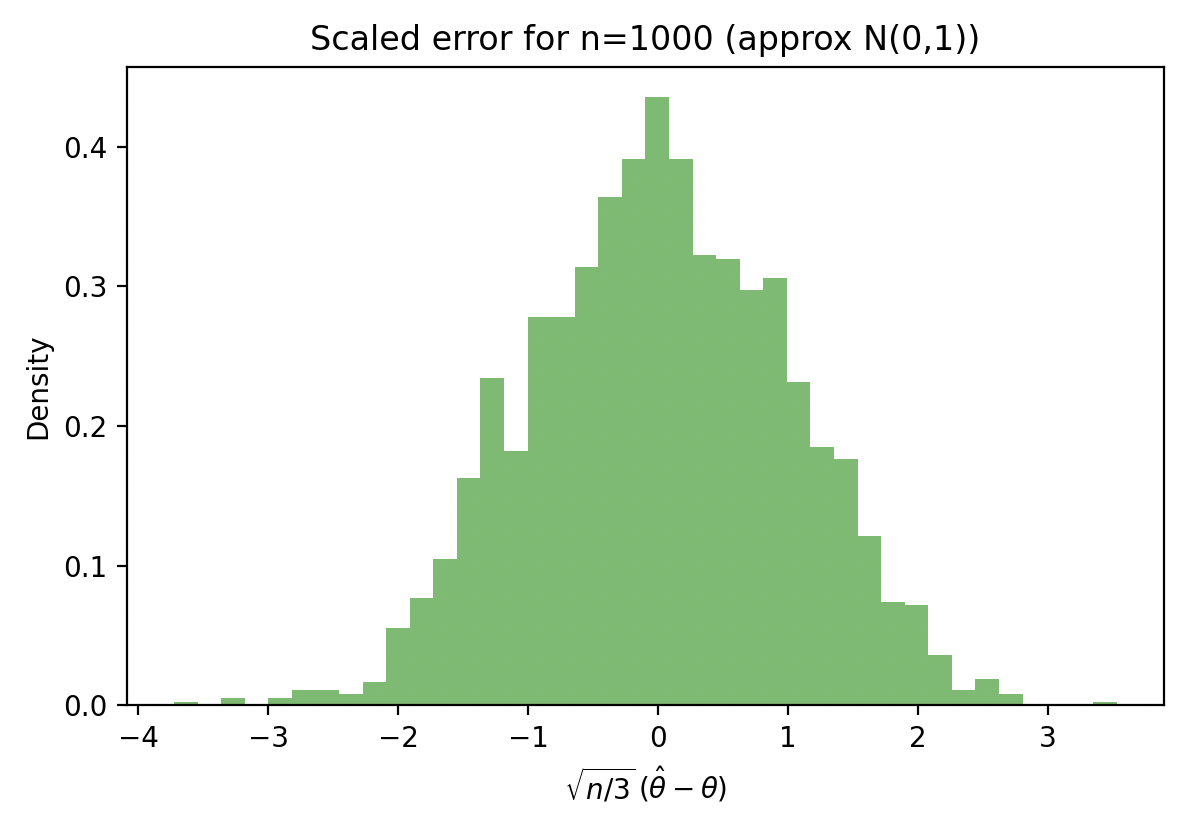
\includegraphics[width=0.5\textwidth]{image2.png}
\end{center}
\begin{center}
    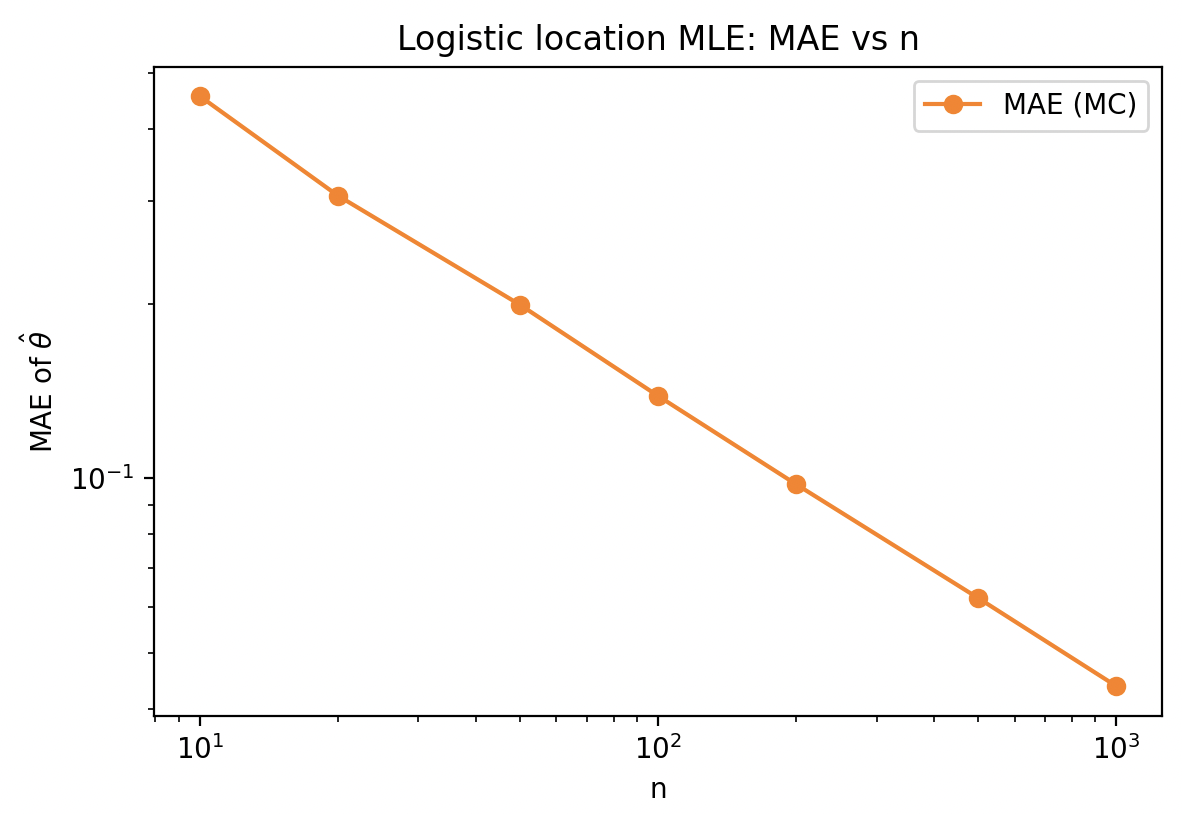
\includegraphics[width=0.5\textwidth]{image3.png}
\end{center}
\begin{center}
    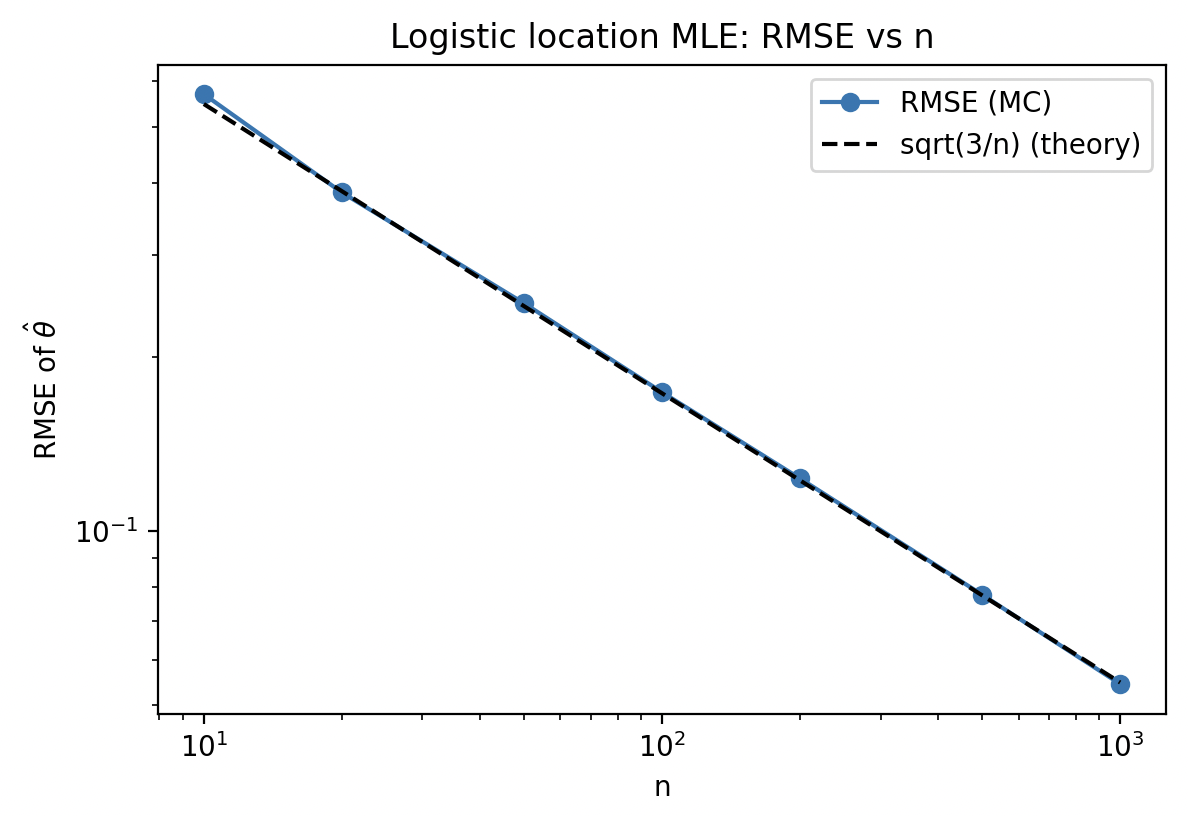
\includegraphics[width=0.5\textwidth]{image4.png}
\end{center}

\newpage

Key formulas: 

Log-likelihood for data $x_1, …, x_n $
\begin{gather*}
    \ell(\theta) = \sum_{i = 1}^{n}\bigg(-(x_i - \theta) - 2\log\Big(1 + \exp\big(-(x_i - \theta)\big)\Big)\bigg)
\end{gather*}
Score: 
\begin{gather*}
    \ell'(\theta) = \sum_{i = 1}^{n}\tanh\left(\frac{x_i - \theta}{2}\right)
\end{gather*}
Hessian: 
\begin{gather*}
    \ell''(\theta) = -\frac{1}{2}\sum_{i = 1}^{n}\text{sech}^2\left(\frac{x_i - \theta}{2}\right) < 0,
\end{gather*}
so the log-likelihood is strictly concave in $\theta $, giving a unique MLE. The MLE solves $\sum_{i = 1}^{n}\tanh\big((x_i - \hat{\theta}) / 2\big) = 0 $

\hfill 

Prove Lemma 3.2

\textbf{Context [MLEs]}: Suppose that our interest is in $g(\theta)$ rather than $\theta $. What is the MLE of $g(\theta)$? To get around techincal difficulties which may occur since one value $\eta = g(\theta)$ may correspond to multiple $\theta $ (if $g $ is not injective) we may assume all the maxima below exist and define the induced likelihood function as
\begin{gather*}
    L^*(\eta):= \underset{\theta\in\{\theta : g(\theta) = \eta\}}{\max}L(\theta)
\end{gather*}
We define the MLE of $g(\theta)$ as 
\begin{gather*}
    \hat{\eta} = \underset{\eta\in\{g(\theta) : \theta\in\Theta\}}{\arg\max} L^*(\eta)
\end{gather*}
The lemma states that: 
\begin{gather*}
    \underset{\eta\in\{g(\theta) : \theta\in\Theta\}}{\max}L^*(\eta) = \max_{\theta\in\Theta}L(\theta)
\end{gather*}

\textbf{Proof:}

Let $\Theta $ be the parameter space, $g: \Theta\to G $, and define for each $\eta $ in the image $g(\Theta)$ the fiber \\$S_\eta := \{\theta\in\Theta : g(\theta) = \eta\}$. By assumption, all displayed maxima exist. 

Upper bound: for any $\eta \in g(\Theta)$,
\begin{gather*}
    L^*(\eta) = \max_{\theta\in S_\eta}L(\theta) \le \max_{\theta\in\Theta}L(\theta)
\end{gather*}
Taking the maximum over $\eta $ on the left yields
\begin{gather*}
    \max_{\eta\in g(\Theta)}L(\theta) \le\max_{\theta\in\Theta}L(\theta)
\end{gather*}
Lower bound: 

Let $\hat{\theta} \in \arg\max_{\theta\in\Theta}L(\theta)$ and set $\hat{\eta} := g(\hat{\theta})\in g(\Theta)$. Since $\hat{\theta} \in S_{\hat{\eta}}$,
\begin{gather*}
    L^*(\hat{\eta}) = \max_{\theta\in S_{\hat{\eta}}}L(\theta) \ge L(\hat{\theta}) = \max_{\theta\in\Theta}L(\theta)
\end{gather*}
Hence
\begin{gather*}
    \max_{\eta\in g(\Theta)}L^*(\eta) \ge \max_{\theta\in\Theta}L(\theta)
\end{gather*}
Combining the two inequalities gives
\begin{gather*}
    \max_{\eta\in g(\Theta)}L^*(\eta) = \max_{\theta\in\Theta}L(\theta)
\end{gather*}
\qed

\end{document}